\chapter{Band gap} \label{sec:BandGapAnalysis}

	All band gaps of our PbS simulations are plotted in figure \ref{fig:BandGap}. Furthermore, we have fitted the $1/R^2$ dependence of
	equation \ref{eq:Bandgap} to all band gaps where no voltage was applied.
	As we can see from the graph, the bulk band gap of \gls{PbS} should approximately be 0.46eV, which means a pretty big deviation
	from experimentally determined values of 0.37eV at 302K (see appendix \ref{sec:PbS}). We have made the same observations while comparing
	other experimental with simulation data. As experimental data, \gls{TEM} images, absorption and \gls{PL} spectra (see figure \ref{fig:PbS_TEM},
	\ref{fig:Abs_PbS} and \ref{fig:PL_PbS}) were available. From the \gls{TEM} images, average particle sizes were measured and compared
	with approximately equivalently sizes from simulations. The results are listed in table \ref{tbl:BandGap}. Significant deviations
	can be noticed between experimental and simulated data, which are reasoned in three significant error sources, that explain the deviations.
	First of all, the synthesis does not deliver perfect spherical and homogeneous \glspl{QD}, which causes the broadening of the spectra.
	Second: it is very difficult to determine the size of the \glspl{QD} from the \gls{TEM} images, especially without
	sophisticated software. This might lead to comparison of experimental and simulated values, that actually do not belong to each other.
	Third: comparing measurements of the real physical world with simulations. There might be errors in the measurement
	apparatus, impurities in the \glspl{QD} and disregarded effects in the simulation, which have an impact in reality.
	
	\begin{table}[htbp]
		\centering
		\begin{tabularx}{\textwidth}{Xc|c|c|c}
															& \multicolumn{4}{c}{Experimental \diameter - Simulated \diameter}														\\
															&	$\sim$ 2.97nm	- 3nm		&	$\sim$ 3.21nm - 3nm &	$\sim$ 3.95nm	-	4nm		&	$\sim$ 4.97nm - 5nm		\\
															&	PbS - 261\footnote{The number is an internal identification for an experiment done in the past.}	& PbS - 61						&	PbS - 190							&	PbS - 220							\\
			\hline
			Energy at \gls{PL} peak	&	1.4529eV 							&	1.2256eV 						&	n/a										&	1.0040eV 							\\
															&	(853nm)								&	(1012nm)						&												&	(1235nm)							\\
			Band gap experimental		&	1.7487eV 							&	1.5194eV 						&	1.2808eV 							&	1.0489eV 							\\
															&	(709nm)								&	(816nm)							&	(968nm)								&	(1182nm)							\\
			Band gap simulated			&	0.9929eV							&	0.9929eV						&	0.8645eV							&	0.7296eV							\\ \\
		\end{tabularx}
		\caption{Comparison of experimental and simulated band gaps.}
		\label{tbl:BandGap}
	\end{table}
	
	\begin{figure}[t]
		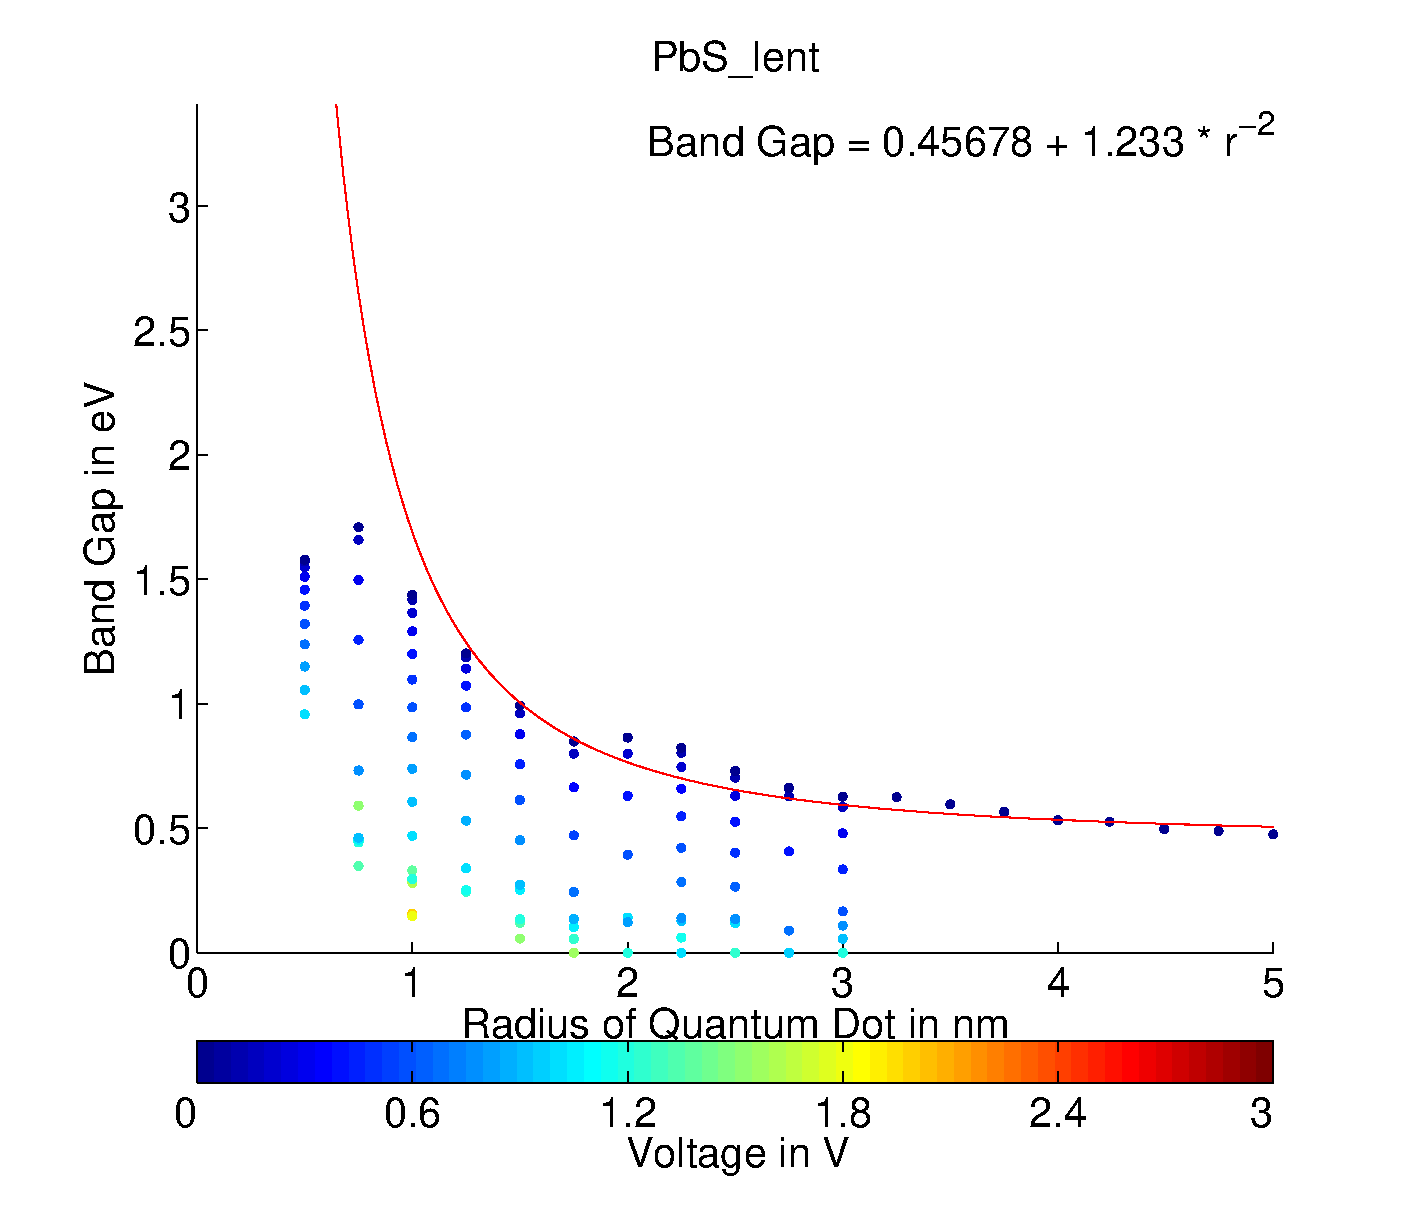
\includegraphics[width=\textwidth]{Fig/Matt_Plots/BandGap}
		\caption{PbS band gaps against radius of all simulated \glspl{QD}. The color indicates the applied voltage.}
		\label{fig:BandGap}
	\end{figure}
	
		\begin{figure}[htpb]
		\centering
		\begin{subfigure}{0.23\textwidth}
			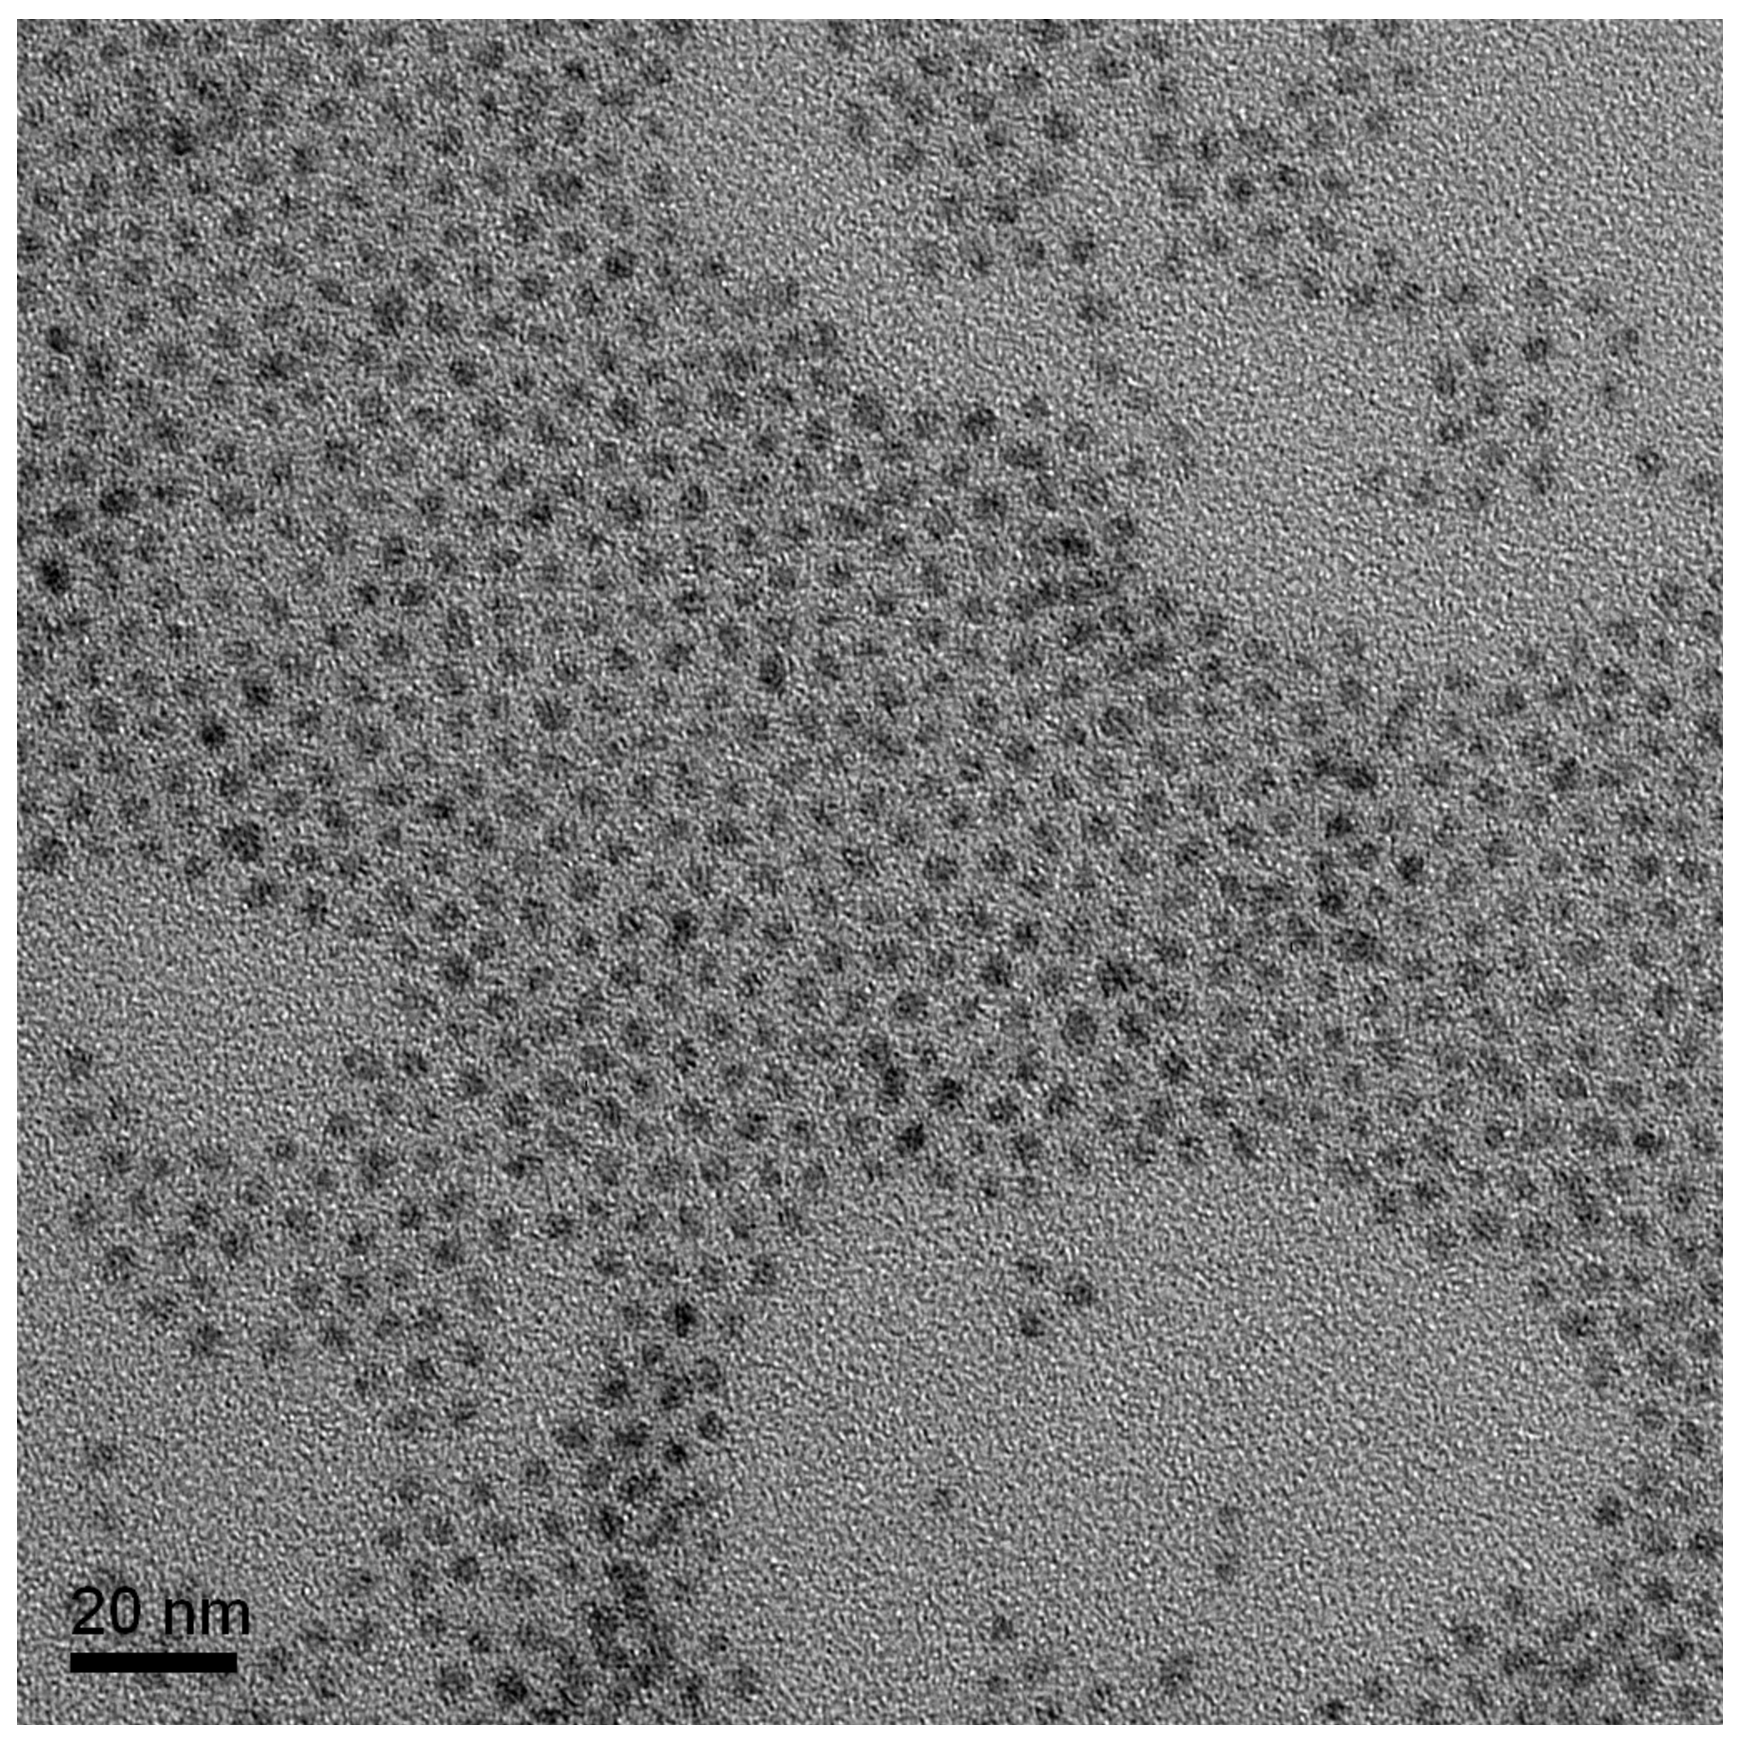
\includegraphics[width=\textwidth]{Fig/Matt_Plots/PbS_190_TEM}
			\caption{PbS - 190, \diameter $\sim$ 3.95nm}
		\end{subfigure}
		\hfill   
		\begin{subfigure}{0.23\textwidth}
			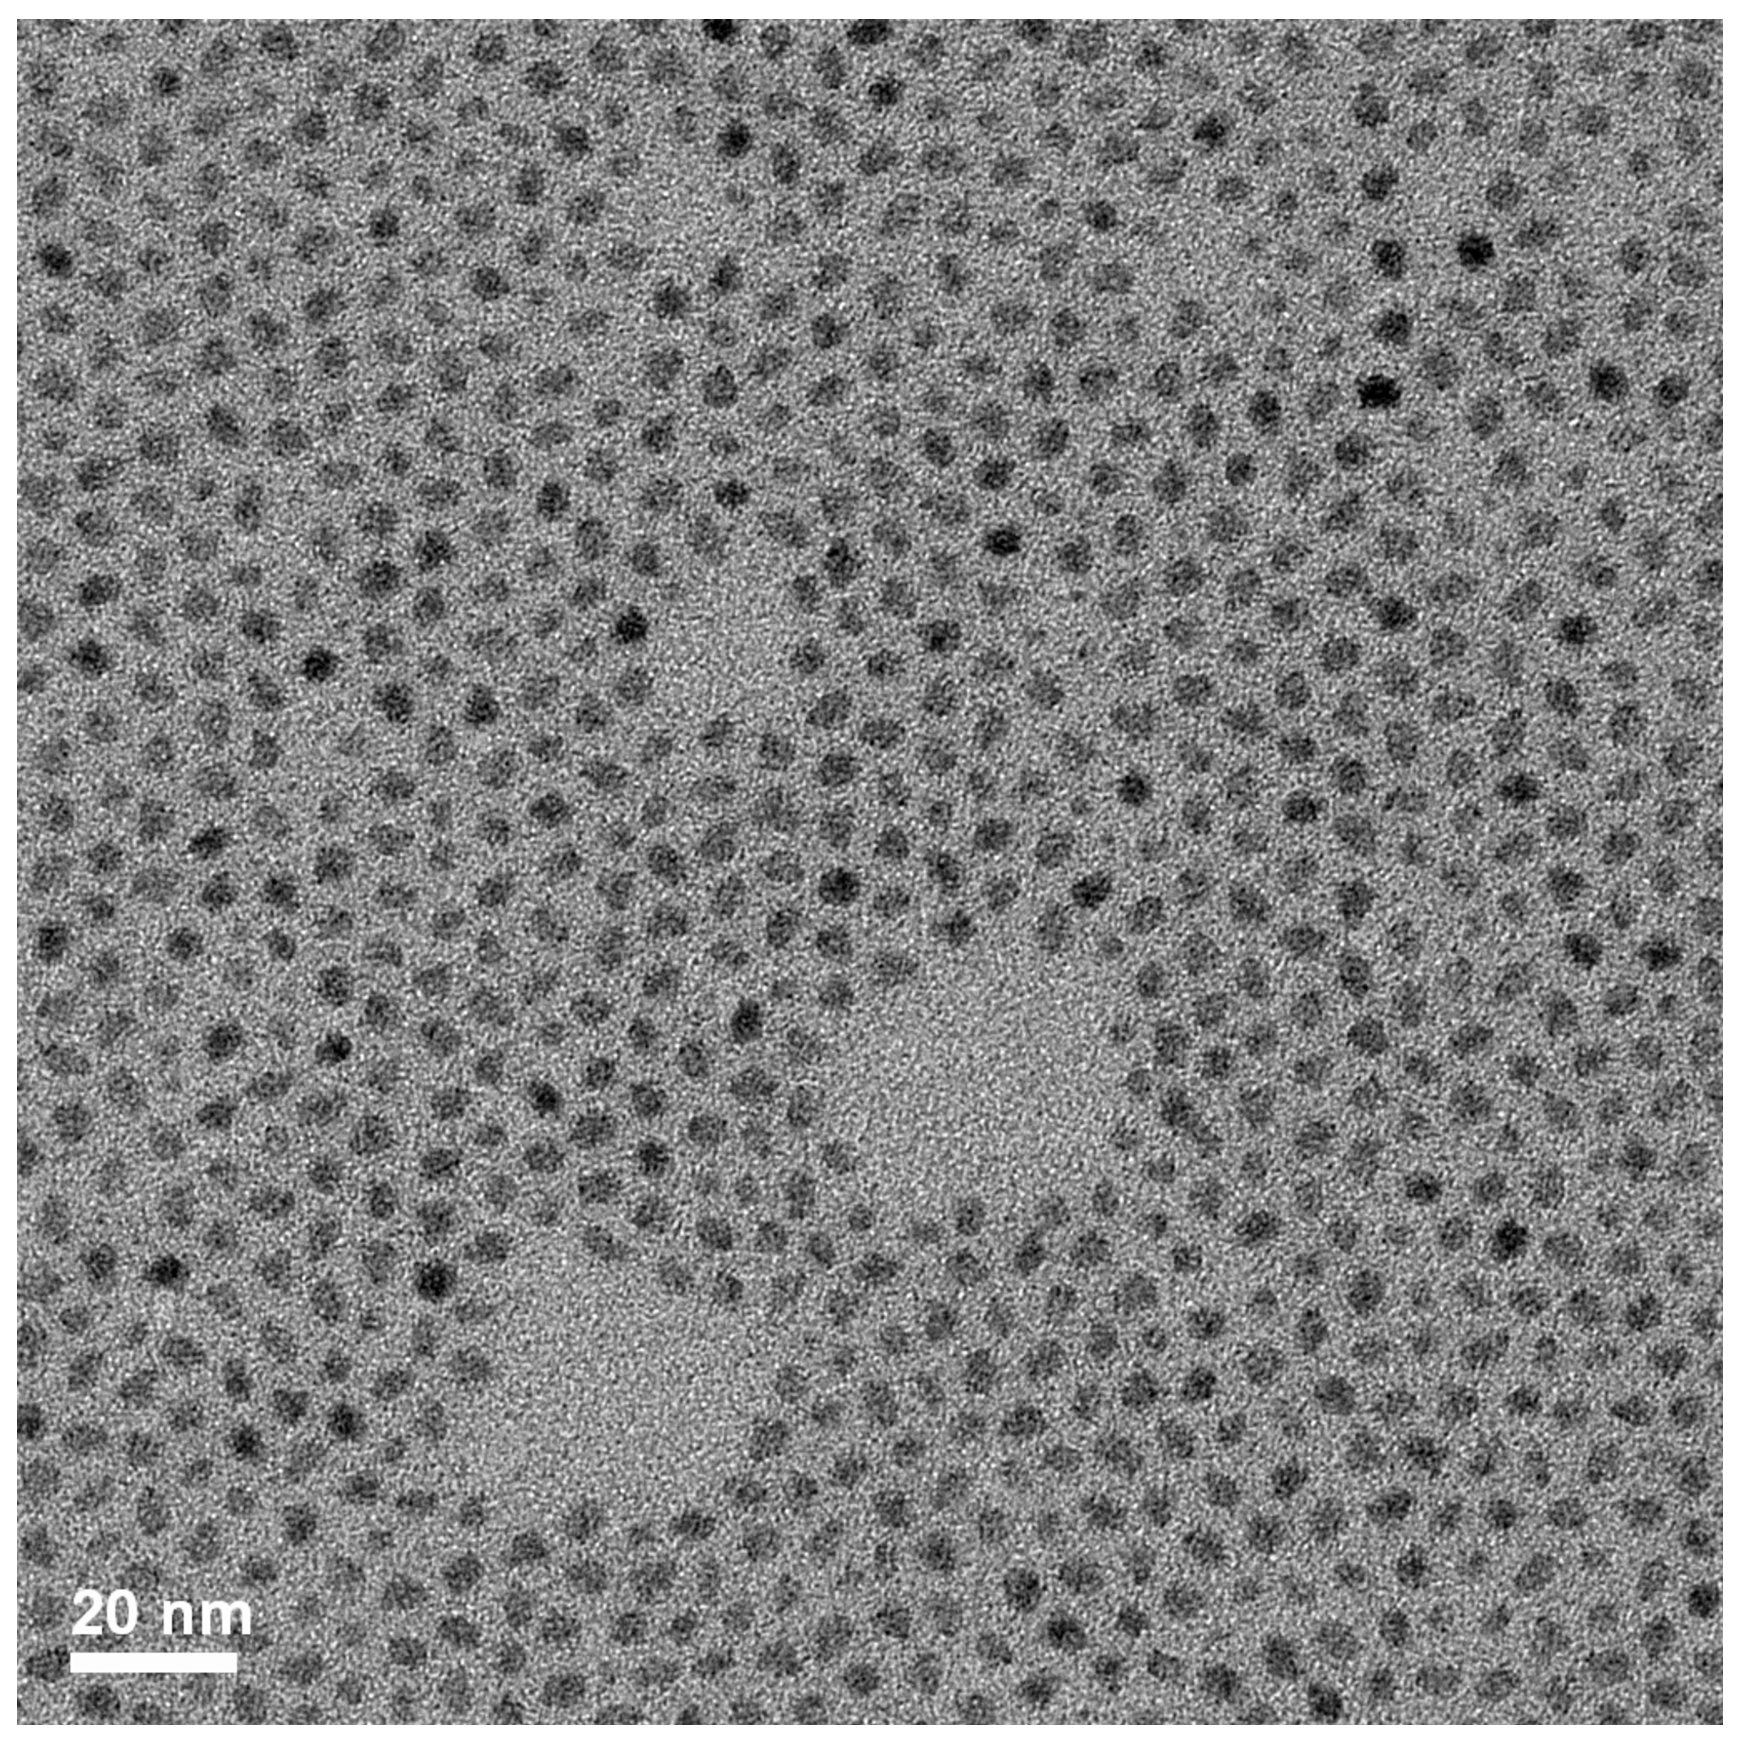
\includegraphics[width=\textwidth]{Fig/Matt_Plots/PbS_220_TEM}
			\caption{PbS - 220, \diameter $\sim$ 4.97nm}
		\end{subfigure}
		\hfill
		\begin{subfigure}{0.23\textwidth}
			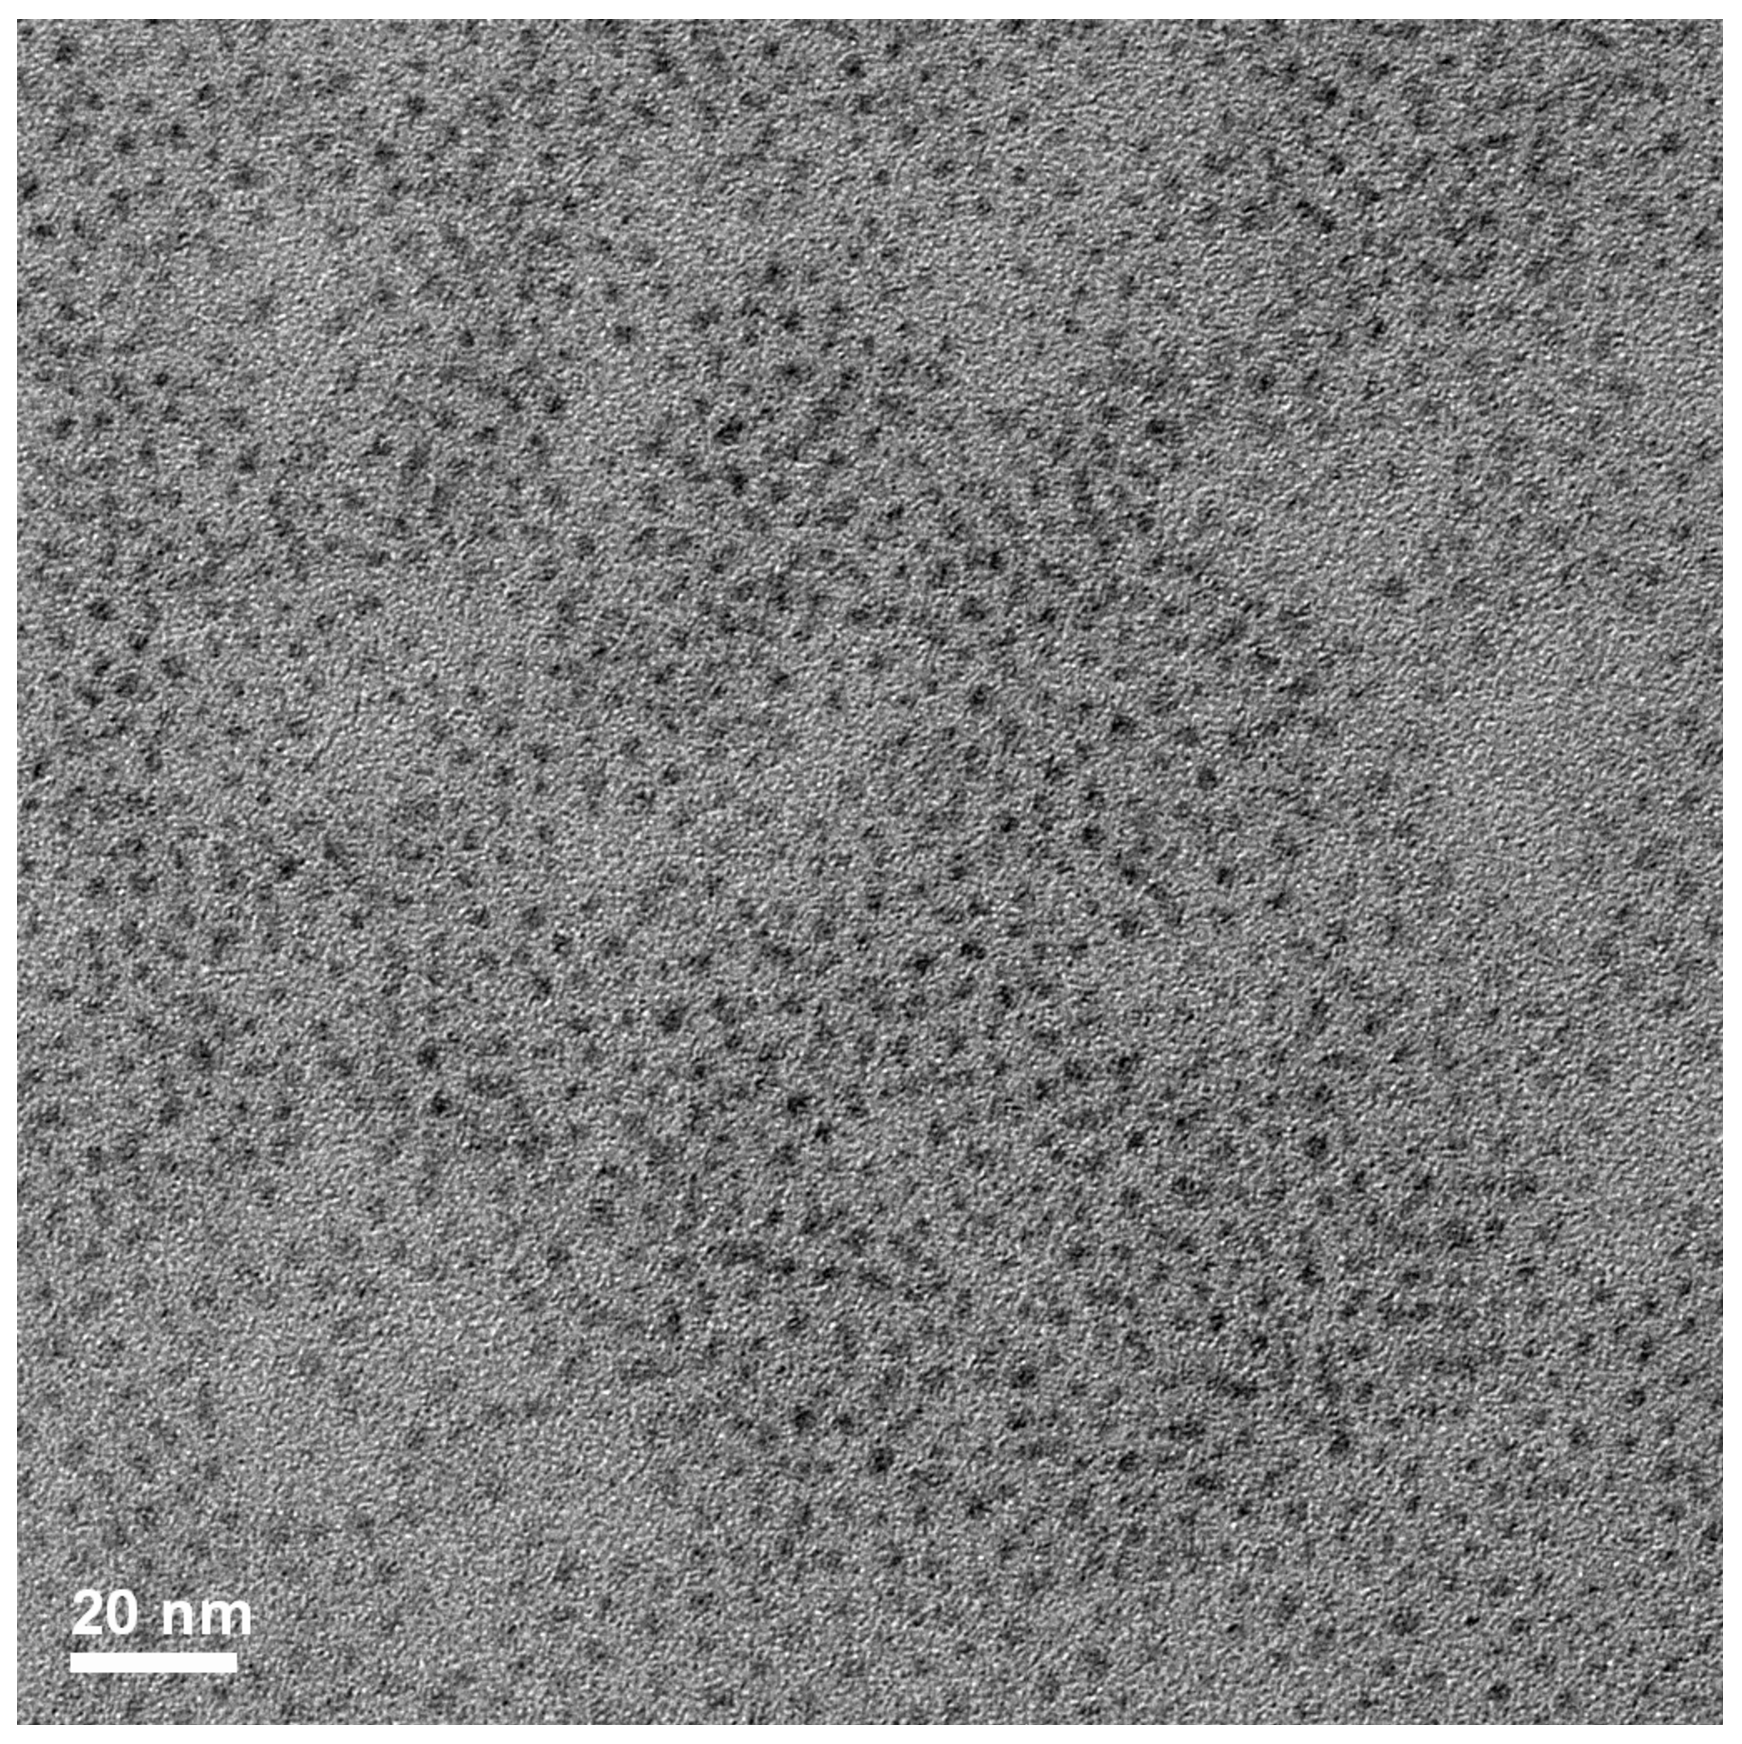
\includegraphics[width=\textwidth]{Fig/Matt_Plots/PbS_261_TEM}
			\caption{PbS - 261, \diameter $\sim$ 2.97nm}
		\end{subfigure}
		\hfill
		\begin{subfigure}{0.23\textwidth}
			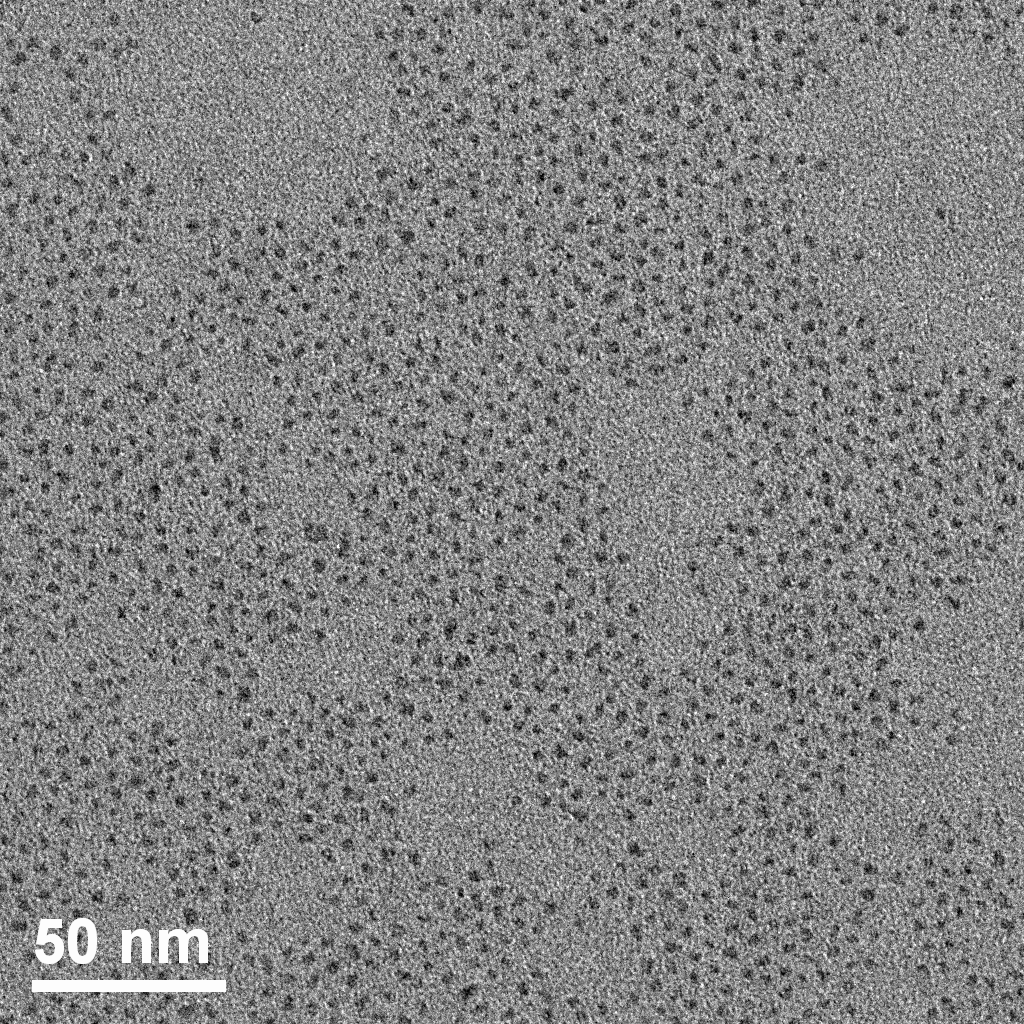
\includegraphics[width=\textwidth]{Fig/Matt_Plots/PbS_61_TEM}
			\caption{PbS - 61, \diameter $\sim$ 3.21nm}
		\end{subfigure}
		\caption{\gls{TEM} images of PbS \glspl{QD}}
		\label{fig:PbS_TEM}	
	\end{figure}

	\begin{figure}[htpb]
		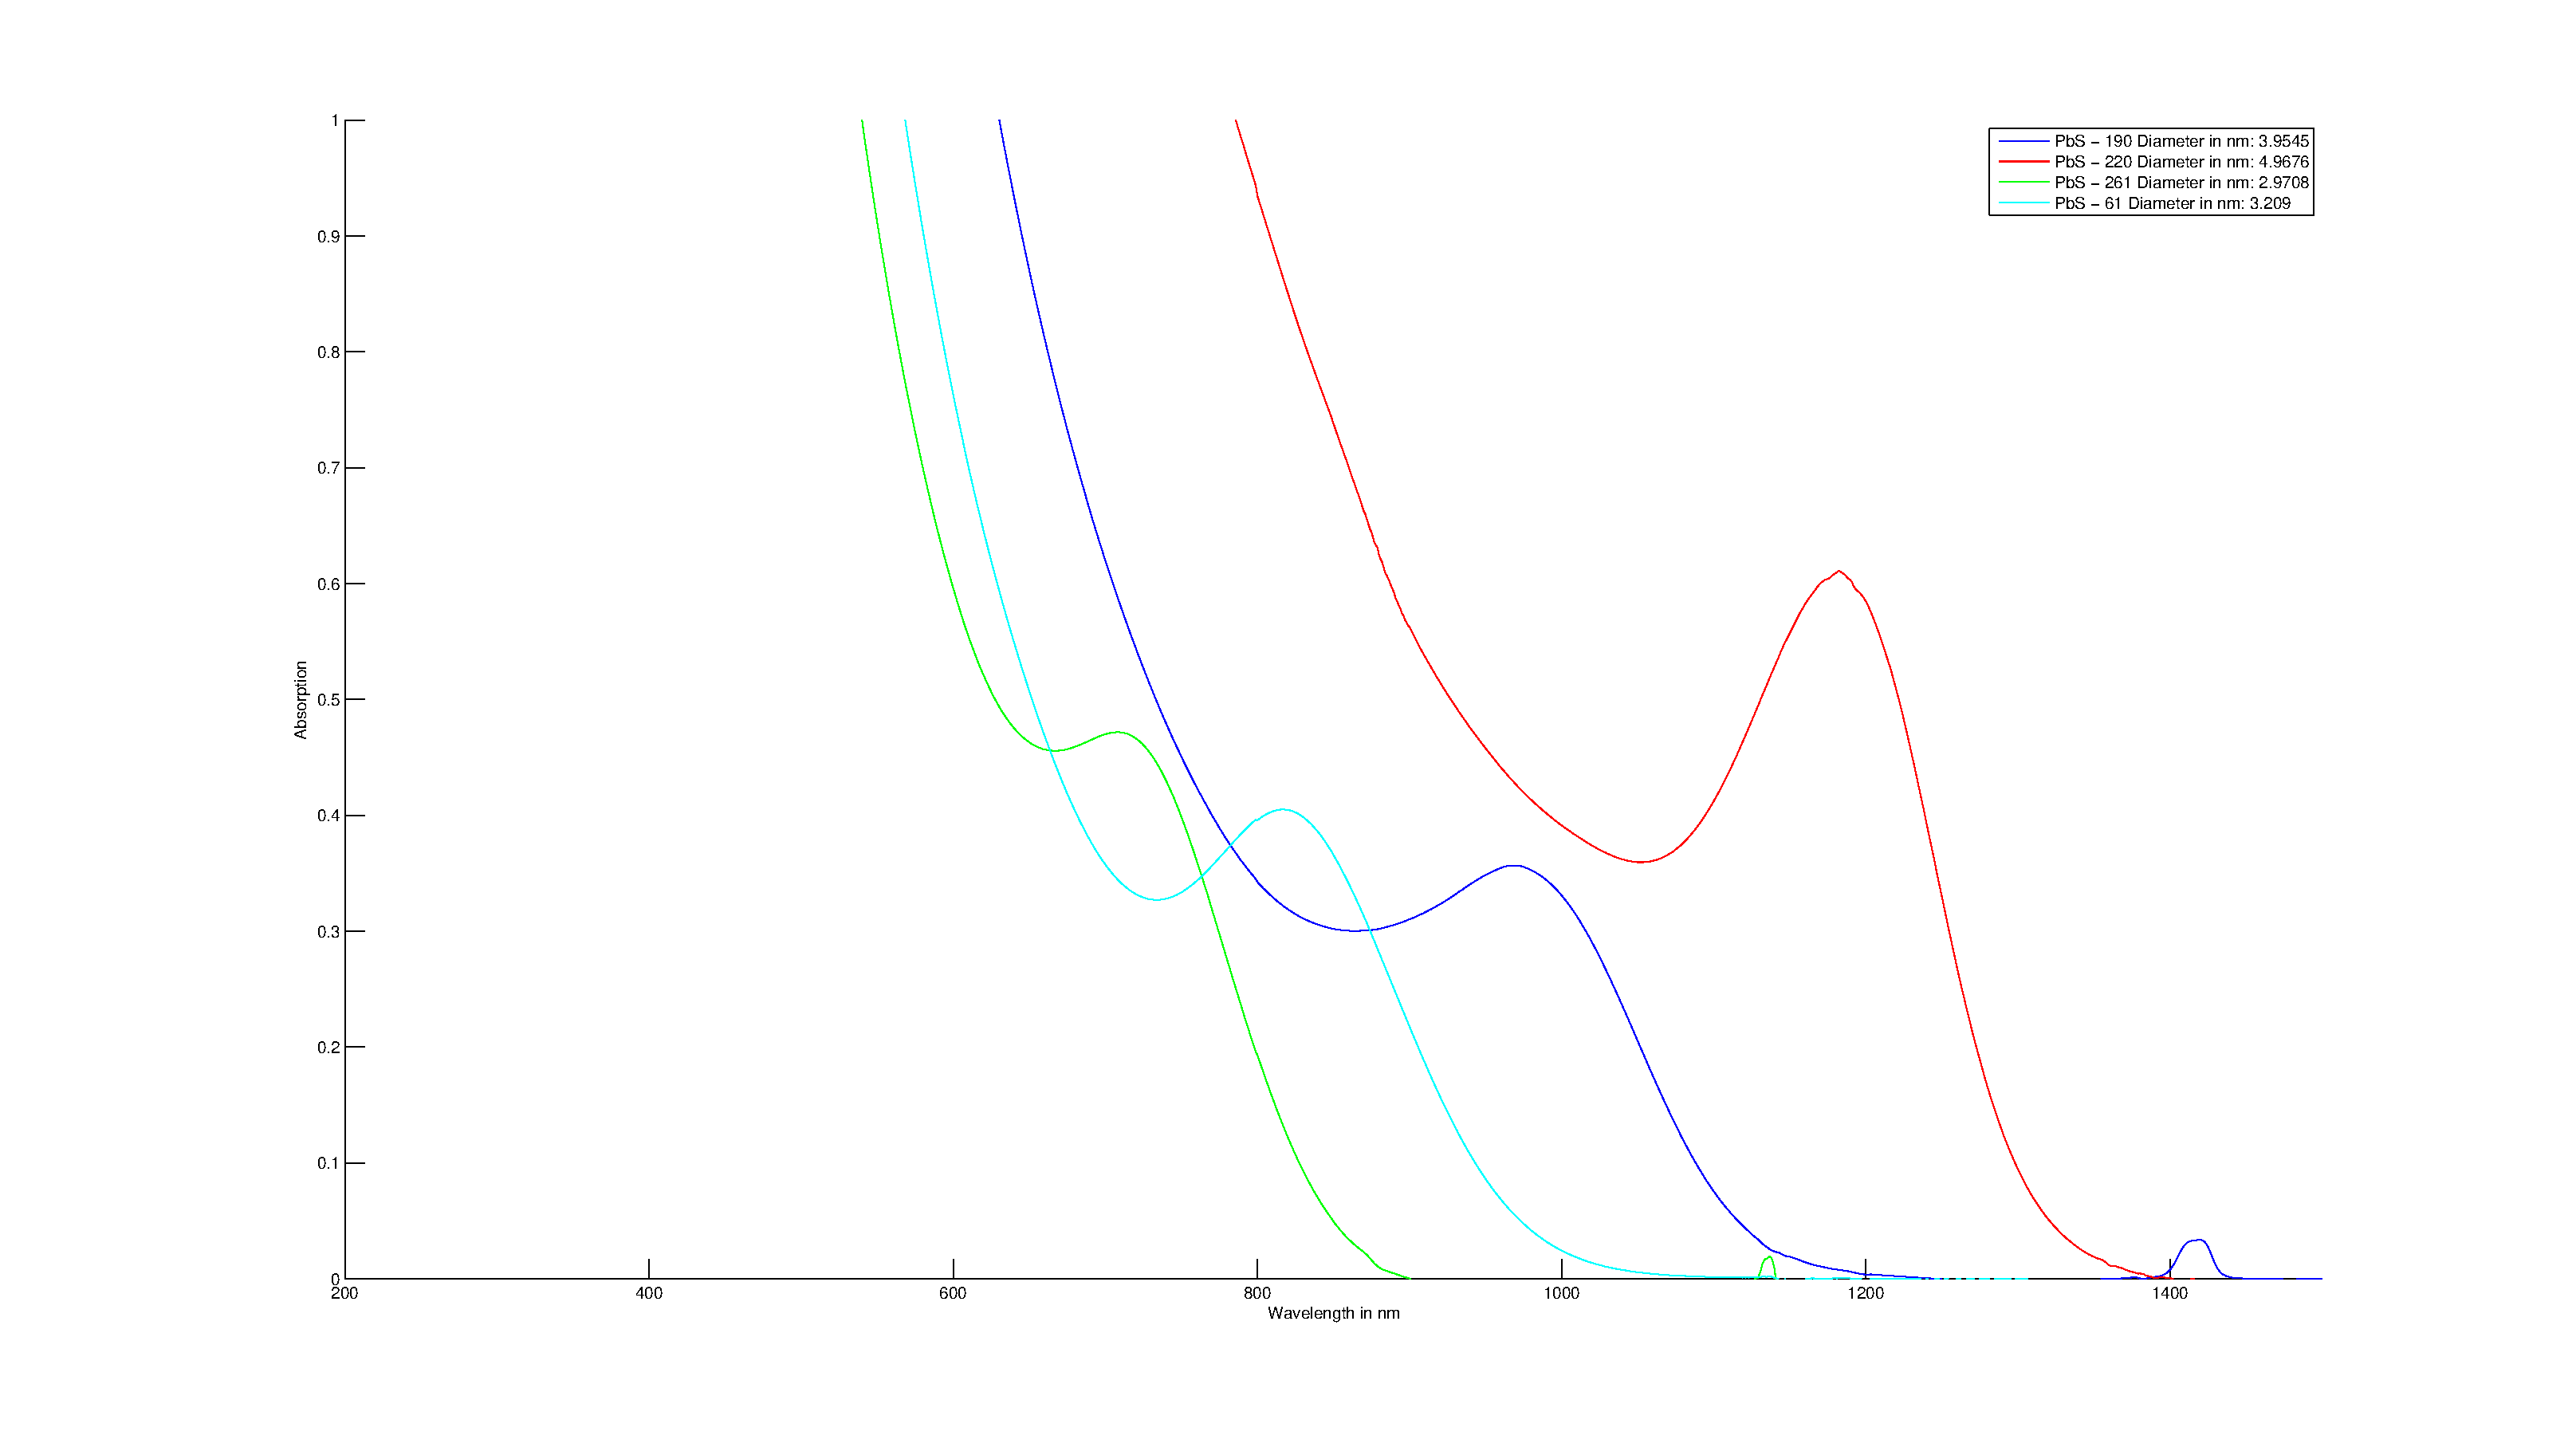
\includegraphics[width=\textwidth]{Fig/Matt_Plots/Abs_PbS}
		\caption{Experimentally determined absorption spectrum plotted against wavelength in nm for 4 synthesized PbS \glspl{QD}.}
		\label{fig:Abs_PbS}
	\end{figure}
	
	\begin{figure}
		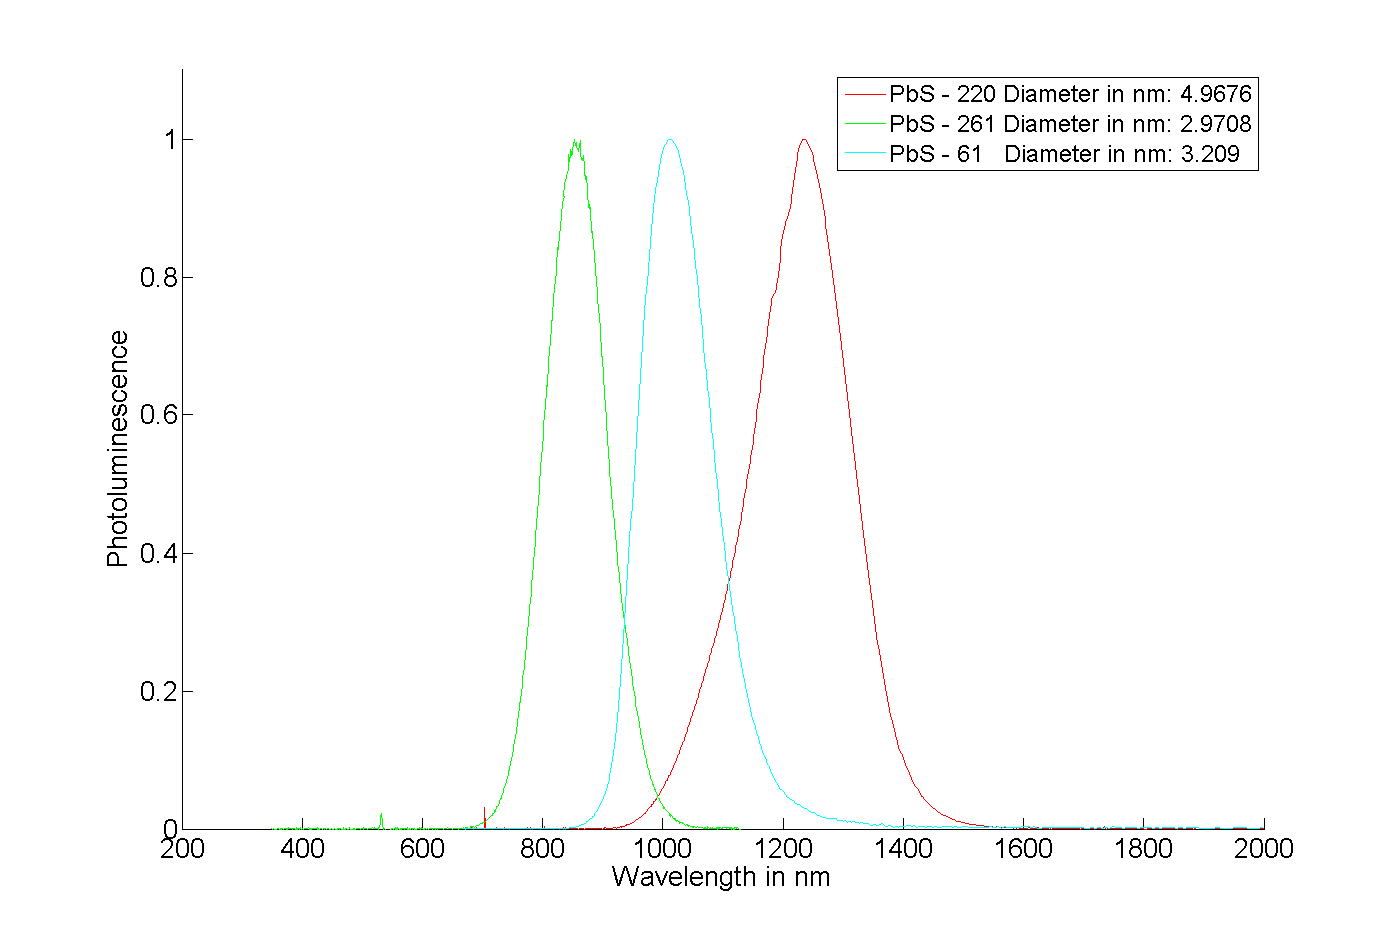
\includegraphics[width=\textwidth]{Fig/Matt_Plots/PL_PbS}
		\caption{Experimentally determined \gls{PL} plotted against wavelength in nm for 3 synthesized PbS \glspl{QD}.}
		\label{fig:PL_PbS}
	\end{figure}
		
	\begin{REMARK}
		All experimental data used in this section were provided by the \gls{LNE} at ETH Zurich.
	\end{REMARK}





\section{Band gap of QDs in presence of an applied voltage}
	
	In figure \ref{fig:EnergyLevels} we see, that with increasing voltage the band gaps approach a zero value. Interestingly, this does not happen linearly, 
	for every constant voltage increment.	Visualizing this effect for constant radii (figure \ref{fig:BandGap_Volt}), we recognize that the energy gap drops in a	parabolic way until it completely reaches the zero value. Furthermore, we recognize in figure \ref{fig:EnergyLevels_Volt} a shift of all energy levels towards each other.
	\begin{figure}
		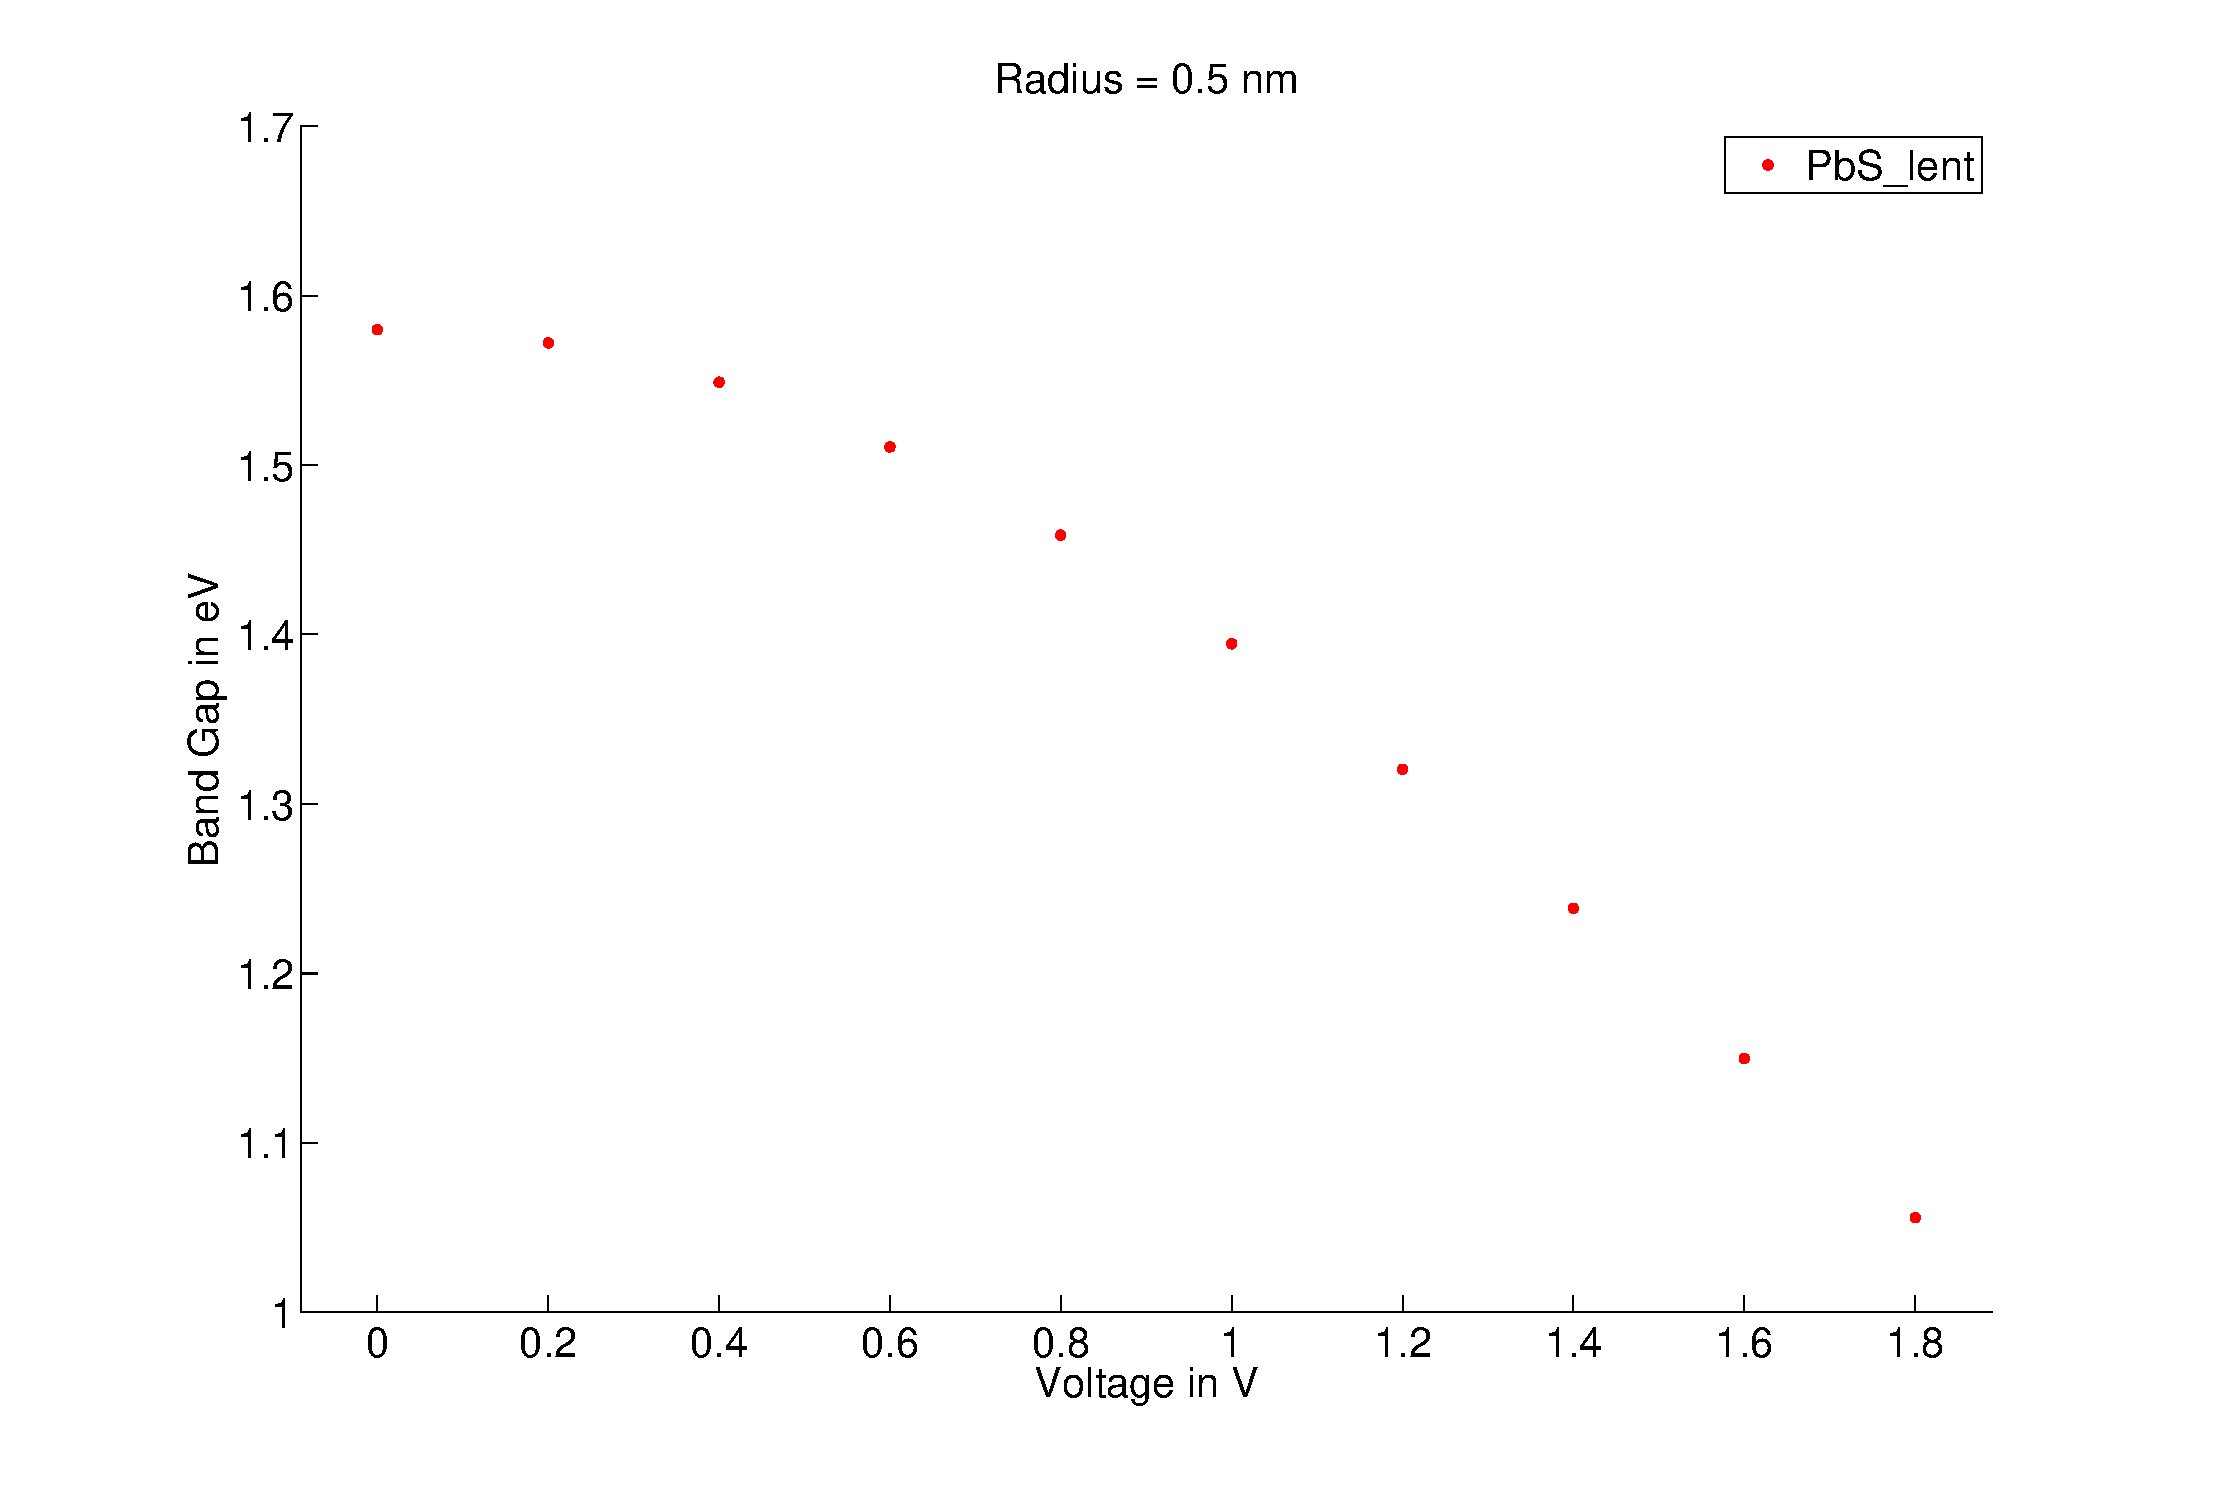
\includegraphics[width=\textwidth]{Fig/Matt_Plots/BandGap_Volt}
		\caption{PbS band gaps plotted against voltage with constant radius 0.5nm.}
		\label{fig:BandGap_Volt}
	\end{figure}
	\begin{figure}
		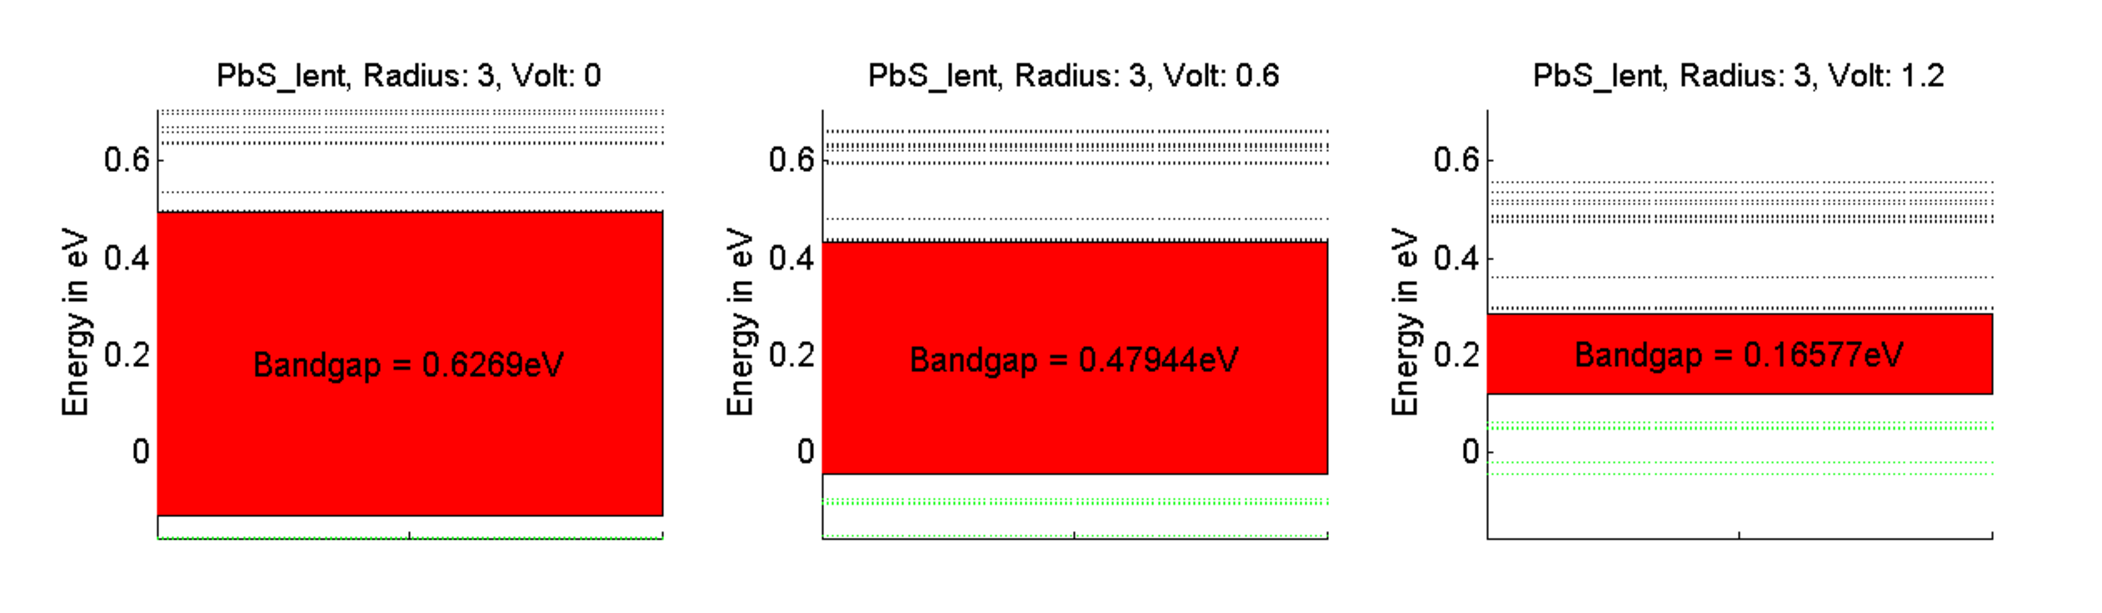
\includegraphics[width=\textwidth]{Fig/Matt_Plots/EnergyLevels}
		\caption{PbS energy levels for different voltages with constant radius 3nm.}
		\label{fig:EnergyLevels_Volt}
	\end{figure}
	